\documentclass{article} 
	\usepackage{fontspec,booktabs,xunicode,xltxtra,amsmath,amssymb,caption,colortbl,float,caption,algorithm,algpseudocode}
	\usepackage{graphicx}
	\usepackage{pgfplots}
	\usepackage{xeCJK}
	\setCJKmainfont{MSYH.ttc}
	\title{人工智能\\Square loss与logistic loss的比较}
	\author{孔静-2014K8009929022}

\begin{document}   
	\maketitle
	\tableofcontents
	\newpage
	\section{问题}\
	
		构造X为2维的2分类数据(0, 1),计算线性分类的直线和Logistic Regression的分类直线(考虑正则化L2),说明Logistic Regression的鲁棒性
	\section{分析}
		\subsection{线性回归}\
			
			估计函数\[{\rm{h}}(x) = {h_\theta }(x) = {\theta _0}{x_0} + {\theta _1}{x_1} = {\theta ^T}X,({x_0} = 1)\]
			
			损失函数\[J(\theta ) = \frac{1}{{2n}}\sum\limits_{i = 1}^n {{{[{h_\theta }({x^{(i)}}) - {y^{(i)}}]}^2}} \]
			
			选取梯度下降法\[{\theta _j} = {\theta _j} - \alpha \frac{\partial }{{\partial {\theta _j}}}J(\theta ) = {\theta _j} - \frac{\alpha }{n}\sum\limits_{i = 1}^n {[{h_\theta }({x_i}) - {y_i}]} x_i^j\]
			
			得到结果
		\subsection{逻辑回归}\
		
			假设函数\[\begin{array}{l}
			{h_\theta }(x) = g({\theta ^T}x) = \frac{1}{{1 + {e^{ - {\theta ^T}}}x}}\\
			g(z) = \frac{1}{{1 + {e^{ - z}}}}
			\end{array}\]
			
			损失函数\[\begin{array}{*{20}{l}}
			{J(\theta ) = \frac{1}{n}\sum\limits_{i = 1}^n {{\rm{Cos}}t({h_\theta }({x_i}),{y_i})} }\\
			{ =  - \frac{1}{n}\sum\limits_{i = 1}^n {[{y_i}\log } {h_\theta }({x_i}) + (1 - {y_i})\log (1 - {h_\theta }({x_i}))]}
			\end{array}\]
			
			L2正则化的损失函数\[J(\theta ) = \frac{1}{{2n}}\sum\limits_{i = 1}^n {{{[{h_\theta }({x^{(i)}}) - {y^{(i)}}]}^2}} {\rm{ + }}C\sum\limits_{i = 1}^n {\theta _j^2} \]
			
			梯度下降法\[{\theta _j} = {\theta _j} - \alpha \frac{\delta }{{{\delta _{{\theta _j}}}}}J(\theta ) = {\theta _j} - \frac{\alpha }{n}(\sum\limits_{i = 1}^n {({h_\theta }({x_i}) - {y_i})x_i^{(j)}}  - C{\theta _j})\]
			
			得到结果
	\section{结果}\
		\subsection{无异常点}
			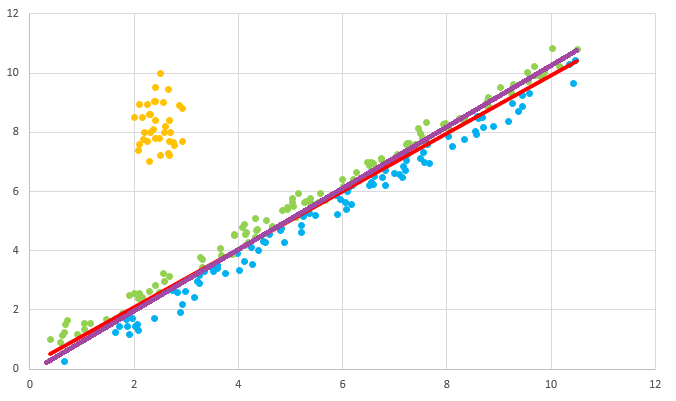
\includegraphics[scale=1.1]{0.png}
		\subsection{有异常点}
			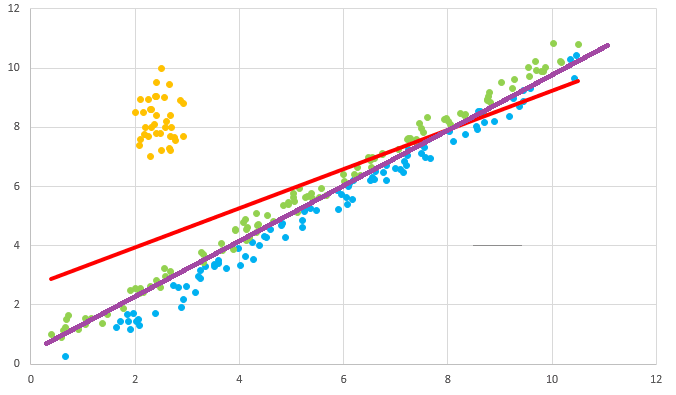
\includegraphics[scale=1.1]{1.png}
		\subsection{分析结果}\
		
			黄点为异常点,正常数据为绿点和蓝点,绿点和黄点同为class1类,蓝点为class0类,红线为线性回归,紫线为逻辑回归。从下两图,可明显看出,当不加入异常点时,两者均与实际差不多;加入异常点时,线性回归偏转较大,并不正确,逻辑回归因为异常数据有偏转,但仍能体现数据分布,可见其鲁棒性。
		

	\end{document}
\end{document}